\chapter[Test e Performance]{Test e Performance}

La letteratura descritta nel secondo capitolo giunge a una conclusione concorde sui benchmark per i gestori di memoria dinamicamente allocata: per valutare un algoritmo di allocazione, è necessario osservarne il comportamento all’interno di un contesto realistico. Ciò può avvenire solamente laddove le tracce adoperate per condurre i benchmark siano vicine alle allocazioni realmente compiute da programmi reali, che sono presi come esempio (esistono utilities che permettono di registrare le richieste, in modo da poterle usare a questo scopo).

Quando le tracce sono casualmente generate, il risultato finale ci dice ben poco sulle capacità effettive dell’allocatore. Le richieste prodotte da un algoritmo probabilistico creano un modello di comportamento, ma questo non è sufficiente: riprodurre le complesse interazioni tra allocazioni e deallocazioni di memoria è molto difficile, poiché queste ultime sono poco comprese e differiscono grandemente tra tipologie di applicazione. Il comportamento a fasi dei programmi dà vita a fenomeni di interconnessione sistematica che sono per la maggior parte ignorati.

Nel 1998, Wilson e Johnston approfondiscono i risultati del procedente paper sull’allocazione dinamica di memoria indagando il comportamento di diversi noti programmi scritti in C e C++. Nell’articolo \emph{The Memory Fragmentation Problem: Solved?}~\cite{wilson1998} gli autori tentano di dimostrare come la frammentazione può essere evitata laddove sia scelta con attenzione una politica di allocazione appropriata a prescindere dall’implementazione.

\begin{quote}
``This substantially strengthens our previous results showing that the memory fragmentation problem has generally been misunderstood, and that good allocator policies can provide good memory usage for most programs. The new results indicate that for most programs, excellent allocator policies are readily available, and efficiency of implementation is the major challenge.''

\begin{center}
[...]
\end{center}

``If these results hold up to further study with additional programs, we arrive at the conclusion that the fragmentation problem is a problem of recognizing that good allocation policies already exist, and have inexpensive implementations. For most programs, the problem of simple overheads is more significant than the problem of fragmentation itself.''
\end{quote} 

Il programma è stato sottoposto anche ad analisi attraverso \textit{valgrind}, il popolare programma di \textit{debugging} e \textit{memory analysis}, in particolare adoperando i \textit{tool} \textit{memcheck, massif} e \textit{cachegrind}. Questi strumenti sono stati fondamentali per comprendere in primo luogo se il programma accedesse alla memoria come previsto, e secondariamente per comprendere dove si trovassero le ostruzioni e i punti critici che causavano perdita di efficienza.

\section{Test delle funzionalità}

I test delle funzionalità si concentrano unicamente sulla correttezza del codice: verificano che le funzioni rispondano correttamente a parametri sbagliati o richieste inappropriate. Definendo la flag \lstinline|DEBUG| a tempo di compilazione abbiamo accesso a maggiori informazioni sugli errori e sulle loro cause. 

\subsection{SlabAllocator}
\begin{table}[H]
\centering
\begin{tabularx}{\textwidth}{|l|X|}
\hline
\textbf{Nome del Test} & \textbf{Descrizione} \\
\hline
\texttt{test\_invalid\_init} & Verifica che l'allocatore gestisca correttamente parametri di inizializzazione non validi (es. dimensione zero o numero massimo di slab non valido). \\
\hline
\texttt{test\_create\_destroy} & Controlla che la creazione e distruzione di uno slab avvengano correttamente, senza memory leak o errori. \\
\hline
\texttt{test\_alloc\_pattern} & Testa il comportamento dell'allocatore con un pattern di allocazioni e deallocazioni ripetute per verificare la correttezza della gestione della memoria. \\
\hline
\texttt{test\_exhaustion} & Verifica il comportamento quando lo slab è pieno (es. ritorno di NULL o gestione degli errori quando non c'è più memoria disponibile). \\
\hline
\texttt{test\_invalid\_free} & Controlla come l'allocatore gestisce la deallocazione di puntatori non validi (es. NULL o indirizzi non allocati). \\
\hline
\end{tabularx}
\caption{Test funzionali per SlabAllocator}
\end{table}

I test per lo SlabAllocator sono generalmente semplici in natura: poiché la grandezza della richiesta non varia e la lista da gestire è singola, gli unici punti di difficoltà sono la creazione con parametri invalidi o il rilascio di puntatori incorretti.


\subsection{BuddyAllocator e BitmapBuddyAllocator}
\begin{table}[H]
\centering
\begin{tabularx}{\textwidth}{|l|X|}
\hline
\textbf{Nome del Test} & \textbf{Descrizione} \\
\hline
\texttt{test\_invalid\_init} & Verifica che l'allocatore gestisca correttamente inizializzazioni non valide (es. dimensione zero, parametri NULL, o valori non supportati). \\
\hline
\texttt{test\_create\_destroy} & Testa la corretta creazione e distruzione di un allocatore, assicurandosi che non ci siano memory leak o corruzione dei dati. \\
\hline
\texttt{test\_single\_allocation} & Verifica che l'allocatore possa rispondere correttamente ad allocazioni invalide e gestire correttamente una singola allocazione. \\
\hline
\texttt{test\_multiple\_allocation} & Controlla il comportamento dell'allocatore quando vengono effettuate più allocazioni consecutive, assicurandosi che tutte abbiano successo e non si sovrappongano. \\
\hline
\texttt{test\_varied\_sizes} & Testa l'allocazione di blocchi di dimensioni diverse per verificare che l'allocatore gestisca correttamente richieste eterogenee. \\
\hline
\texttt{test\_buddy\_merging} & Verifica che, dopo una serie di allocazioni e deallocazioni, l'allocatore riesca a fondere correttamente i blocchi liberi adiacenti (buddy merging) per evitare frammentazione. \\
\hline
\texttt{test\_invalid\_reference} & Controlla come l'allocatore gestisce tentativi di deallocazione di riferimenti non validi (es. NULL, doppio free, o puntatori non allocati). \\
\hline
\end{tabularx}
\caption{Test funzionali per BuddyAllocator e BitmapBuddyAllocator}
\end{table}

Gli allocatori che accettano richieste a taglia variabile presentano una complessità maggiore rispetto a quelli a taglia fissa, poiché devono gestire dinamicamente la suddivisione e la fusione dei blocchi di memoria per rispondere a richieste di dimensioni differenti. Questo comporta una maggiore probabilità di introdurre errori nella gestione della memoria come la perdita di riferimenti o la mancata fusione dei blocchi liberi (\emph{buddy merging}). I test svolgono un ruolo fondamentale nell'evidenziare anomalie e comportamenti indesiderati

Oltre ai test elencati, è utile prevedere casi limite e scenari di stress, come sequenze di allocazioni e deallocazioni ripetute con dimensioni variabili, tentativi di allocazione che saturano la memoria disponibile, e la verifica della corretta gestione di errori (ad esempio, \emph{double free} o allocazioni fuori dai limiti consentiti).

\section{Benchmark}
Poiché la nostra analisi si concentra principalmente sulla correttezza dell'implementazione, i test sopra delineati forniscono una prima conferma del nostro operato. Tuttavia, l'importanza della \textit{performance} dell'allocatore in diversi casi applicativi risulta essenziale per poter veramente trarre delle conclusioni a riguardo. 
Nel corso delle ricerche, l'articolo \textit{"Designing a Trace Format for Heap Allocation Events"}~\cite{chilimbi2000} di T.Chilimbi et al ha fornito un'interessante base teorica per il parser qui descritto. Tuttavia, il nostro vuole essere unicamente un prototipo di funzionamento al fine di svolgere analisi più profonde, e sicuramente fornisce ben poche delle capacità descritte nell'articolo o altrimenti rese disponibili da altri strumenti simili applicati nel campo.\footnotemark

\footnotetext{Alcuni di questi che menzioniamo per dovere di cronaca sono \texttt{perf, LTTng} e \texttt{ETW}. }

Per facilitare dunque l’analisi del comportamento degli allocatori in presenza di pattern complessi di allocazione e deallocazione, è stata introdotta una funzionalità che consente di definire facilmente le sequenze di richieste di memoria tramite file di configurazione esterni, senza dover modificare o ricompilare il codice sorgente. In questo modo è possibile variare rapidamente i benchmark e testare diversi scenari. Il codice sorgente di questa funzionalità si trova nei moduli \texttt{benchmark} e \texttt{parse}.

Ciò è reso possibile dall’implementazione da parte di ogni allocatore dell’interfaccia \texttt{<Allocator>}. Poiché abbiamo a nostra disposizione i puntatori alle funzioni necessarie per svolgere tutte le operazioni, possiamo standardizzare il funzionamento delle classi dividendole in due categorie: allocatori a taglia fissa, che permettono di richiedere blocchi di grandezza prestabilita (e.g. \texttt{SlabAllocator}) e allocatori a taglia variabile, ossia le classi "figlie" di \texttt{VariableBlockAllocator}, le quali invece lasciano all’utente la scelta della dimensione dell’area di memoria richiesta (ossia \texttt{BuddyAllocator} e \texttt{BitmapBuddyAllocator}, nella nostra implementazione).

\begin{lstlisting}
  // template per allocatore a dimensione fissa
  void *FixedSizeAllocator_malloc(FixedSizeAllocator *a);
  void *FixedSizeAllocator_free(FixedSizeAllocator *a);
  // template per allocatore a dimensione variabile
  void *VariableSizeAllocator_malloc(VariableSizeAllocator *a, size_t size);
  void *VariableSizeAllocator_free(VariableSizeAllocator *a)
\end{lstlisting}

Il programma cerca all’interno della cartella \texttt{./benchmarks} file che abbiano l’estensione \texttt{.alloc}. Modificando il testo al loro interno si possono definire la tipologia di allocatore, i suoi parametri di inizializzazione e la sequenza di \texttt{malloc}/\texttt{free} da provare. I comandi sono terminati dal carattere ``a capo'' (\textbackslash n) e le componenti sono divise da una virgola. Comandi che sono preceduti dal carattere percentuale (\%) sono considerati commenti e ignorati.

Vediamo ora come descrivere la classe di allocatore da sottoporre al benchmark e le sue caratteristiche. La prima riga non preceduta da un segno percentuale deve avere necessariamente la seguente struttura: \texttt{i,<allocator class>} dove la classe può essere \texttt{slab}, \texttt{buddy} o \texttt{bitmap}. Il secondo comando informa il programma sui parametri di creazione: \texttt{p,<param1>,<param2>,\ldots}, il numero e il tipo dei quali varia in base alla classe scelta precedentemente.

\begin{table}[H]
\centering
\begin{tabularx}{\textwidth}{|X|X|X|X|}
\hline
\textbf{Allocatore} & \textbf{Dimensione} & \textbf{Parametro 1} & \textbf{Parametro 2} \\
\hline
Slab    & Fissa     & slab\_size   & num\_slabs   \\
\hline
Buddy   & Variabile & memory\_size & max\_levels  \\
\hline
Bitmap  & Variabile & memory\_size & max\_levels  \\
\hline
\end{tabularx}
\caption{Parametri di inizializzazione per ciascuna classe di allocatore}
\end{table}

Per allocare e liberare memoria, l’istruzione deve iniziare rispettivamente con ``a'' o ``f''. Il benchmark per tenere traccia delle allocazioni usa un array avente lunghezza pari al numero massimo possibile di frammenti di memoria. Il comando \texttt{a,<index>} alloca memoria in una posizione specifica dell'array, mentre \texttt{f,<index>} la libera. Nel caso di allocatore a richiesta variabile, dopo l’index dell’array va specificato il numero di byte da allocare (con struttura \texttt{a,<index>,<size>}). 

È fondamentale non allocare più volte sullo stesso indice senza prima liberarlo, altrimenti si perderà il riferimento al puntatore e non sarà più possibile gestirlo correttamente\footnotemark. Il programma esegue la sequenza di \textit{request} e \textit{release}, informa l'utente di eventuali errori e stampa a schermo informazioni sul tempo richiesto: \textit{elapsed\_seconds}, \textit{user\_seconds} e \textit{kernel\_seconds}. In più, produce un file di \texttt{.log} che contiene informazioni sulle singole istruzioni (in particolare, per i\texttt{VariableBlockAllocator}, inserisce anche lo stato della frammentazione interna ed esterna dell'allocatore a ogni istruzione) L'analisi di queste informazioni fornisce alcune metriche aggiuntive sul comportamento dell'allocatore e sulla sua \textit{performance}.

\footnotetext{Il programma di benchmarking non esegue istruzioni che porterebbero alla perdita di un indirizzo e avverte se il benchmark termina senza deallocare tutti gli indirizzi.}

\subsection{Analisi dei pattern di allocazione}
La letteratura sull'argomento ha identificato tre modelli di comportamento principali che possono essere applicati alla maggior parte dei programmi: rampe, picchi e plateau\footnotemark Facciamo riferimento principalmente alla ricerca di Wilson et al., che sottolinea anche come la presenza di un modello nel lungo termine o lungo l'intero ciclo di vita del programma non escluda la presenza di comportamenti osservabili di dimensione minore al suo interno.
\footnotetext{Altri pattern dell'uso di memoria possono essere incontrati, ma sono meno comuni: allo stesso modo, variazioni o combinazioni dei modelli qui citati sono spesso presenti.}
\begin{itemize}
  \item \textbf{Rampe}: molti programmi accumulano determinate strutture dati in modo monotono. Ciò può essere dovuto al fatto che conservano un registro degli eventi o perché la strategia di risoluzione del problema richiede la costruzione di una rappresentazione di grandi dimensioni, dopo la quale è possibile trovare rapidamente una soluzione.
  \item \textbf{Picchi}: molti programmi utilizzano la memoria in modo discontinuo, creando strutture dati relativamente grandi che vengono utilizzate per la durata di una particolare fase e poi la maggior parte o tutte le strutture dati viene scartata. Si noti che le strutture di dati “sopravvissute” sono probabilmente di tipo diverso, perché rappresentano i risultati di una fase, rispetto a valori intermedi che possono essere rappresentati in modo diverso. (Un picco è come una rampa, ma di durata più breve).
  \item \textbf{Plateau}: molti programmi costruiscono rapidamente strutture dati e poi le utilizzano per lunghi periodi (spesso per quasi tutto il tempo di esecuzione del programma).
\end{itemize}

Utilizzando lo strumento da noi creato, siamo in grado di simulare questi pattern e verificare il comportamento degli allocatori in loro presenza. 

\begin{figure}[H]
  \centering
  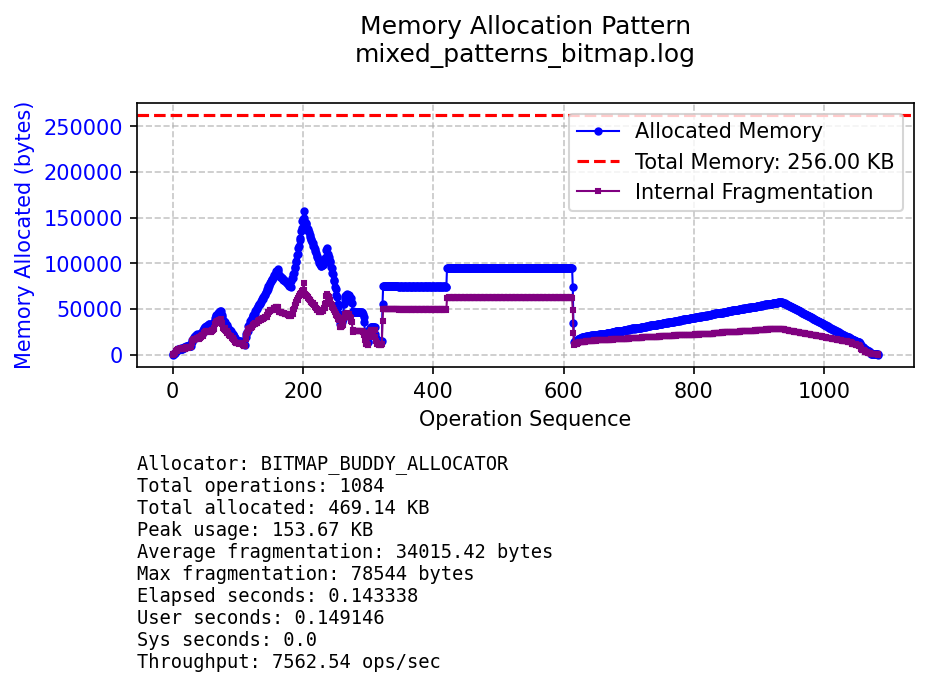
\includegraphics[width=0.9\textwidth]{graphs/mixed_patterns_bitmap.png}
  \caption{Comportamento del BitmapBuddyAllocator su un benchmark contenente in ordine, \textit{peaks, plateaus} e \textit{ramps}.}
  \label{fig:mixed_patterns_bitmap}
\end{figure}



\subsection{Allocazioni sfavorevoli: frammentazione interna}

\begin{figure}[H]
  \centering
  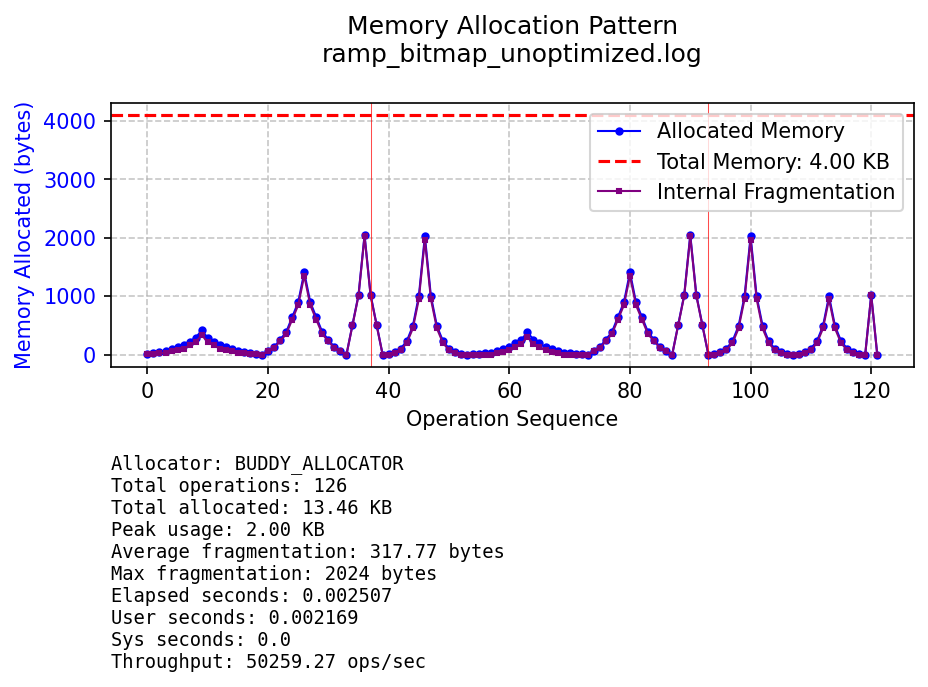
\includegraphics[width=0.9\textwidth]{graphs/ramp_bitmap_unoptimized.png}
  \caption{Sequenza di istruzioni che causano nel BuddyAllocator grande frammentazione interna. Notiamo che la quantità di memoria inutilizzabile è pari a quella allocata.}
  \label{fig:ramp_bitmap_unoptimized}
\end{figure}

\begin{figure}[H]
  \centering
  \begin{minipage}{0.5\textwidth}
    \centering
    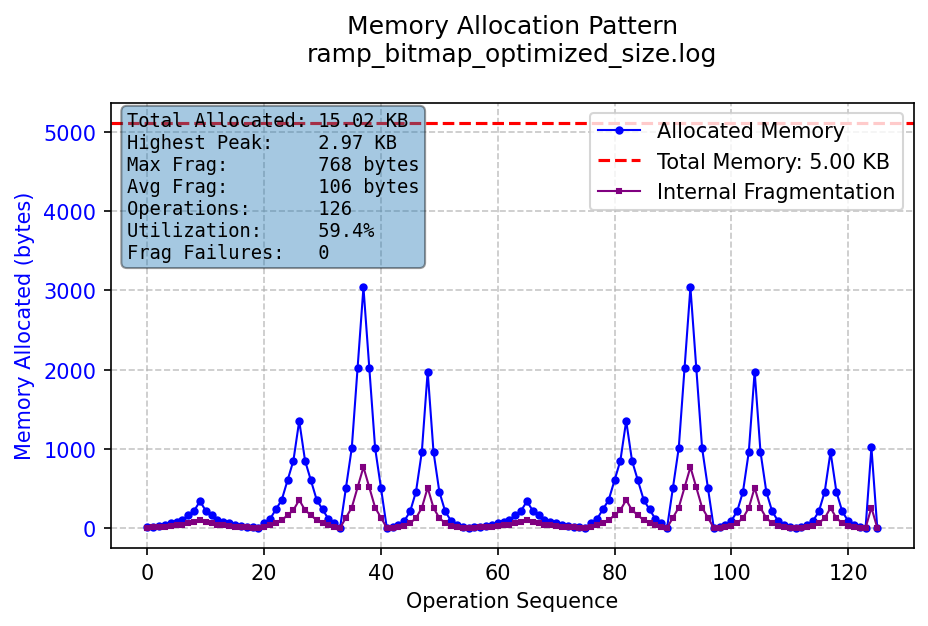
\includegraphics[width=0.95\textwidth]{graphs/ramp_bitmap_optimized_size.png}
    \caption{Con richieste di dimensione leggermente minore, la frammentazione diventa irrilevante.}
    \label{fig:ramp_bitmap_optimized_size}
  \end{minipage}\hfill
  \begin{minipage}{0.5\textwidth}
    \centering
    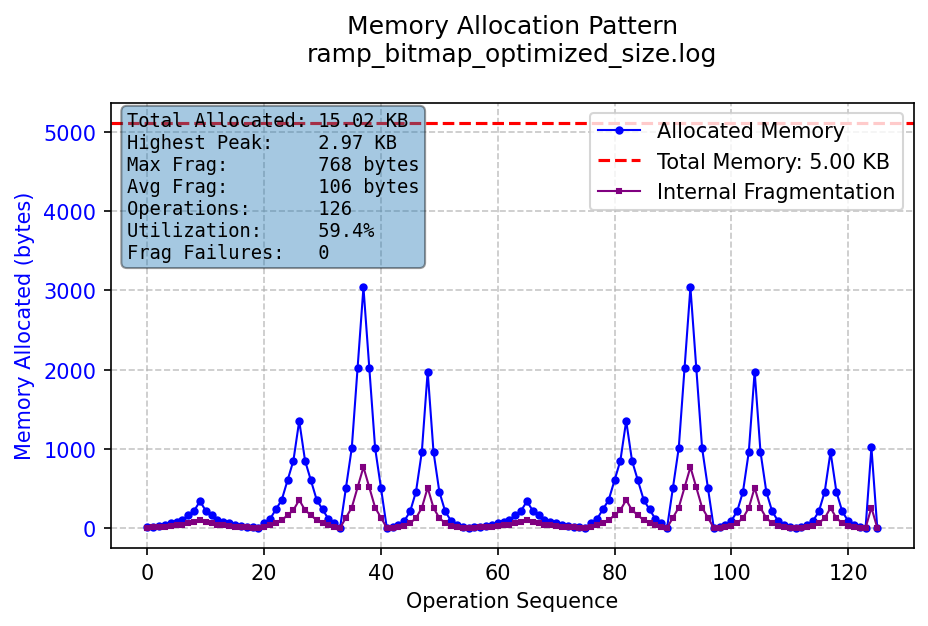
\includegraphics[width=0.95\textwidth]{graphs/ramp_bitmap_optimized_size.png}
    \caption{Allocando relativamente poca memoria in più, la frammentazione diminuisce sostanzialmente.}
    \label{fig:ramp_bitmap_optimized_size}
  \end{minipage}
\end{figure}


\subsection{\textit{LinkedList} e \textit{Bitmap}}
\begin{figure}[H]
  \centering
  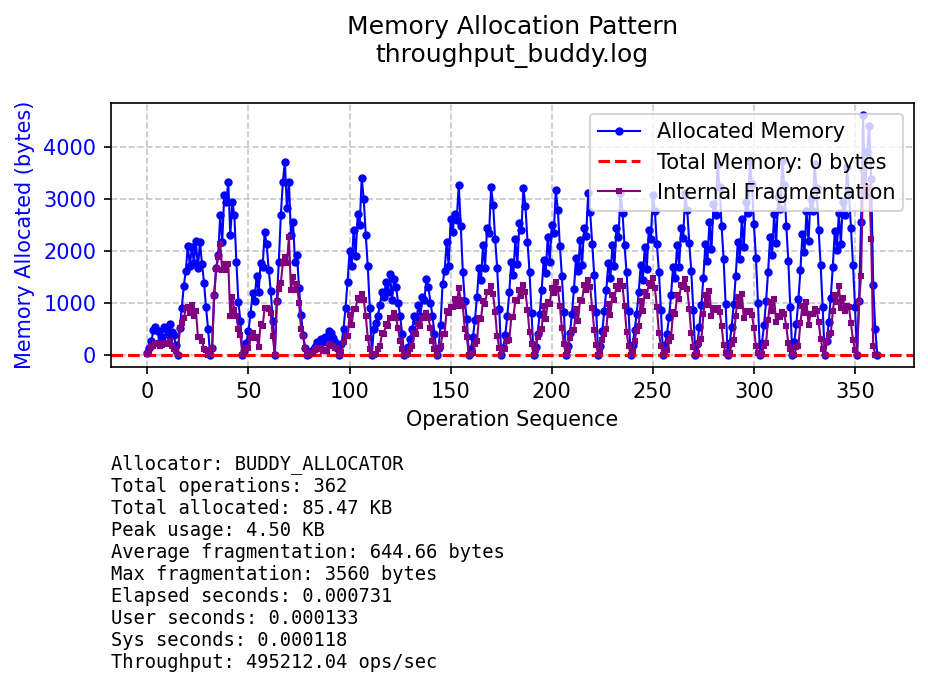
\includegraphics[width=0.9\textwidth]{graphs/throughput_buddy.png}
  \label{fig:throughput_buddy}
\end{figure}
\begin{lstlisting}[language={}]
I refs:        1,992,021
I1  misses:        2,862
LLi misses:        2,436
I1  miss rate:      0.14%
LLi miss rate:      0.12%

D refs:        1,002,895  (736,165 rd   + 266,730 wr)
D1  misses:        4,364  (  2,184 rd   +   2,180 wr)
LLd misses:        3,429  (  1,541 rd   +   1,888 wr)
D1  miss rate:       0.4% (    0.3%     +     0.8%  )
LLd miss rate:       0.3% (    0.2%     +     0.7%  )

LL refs:           7,226  (  5,046 rd   +   2,180 wr)
LL misses:         5,865  (  3,977 rd   +   1,888 wr)
LL miss rate:        0.2% (    0.1%     +     0.7%  )
\end{lstlisting}

\begin{figure}[H]
  \centering
  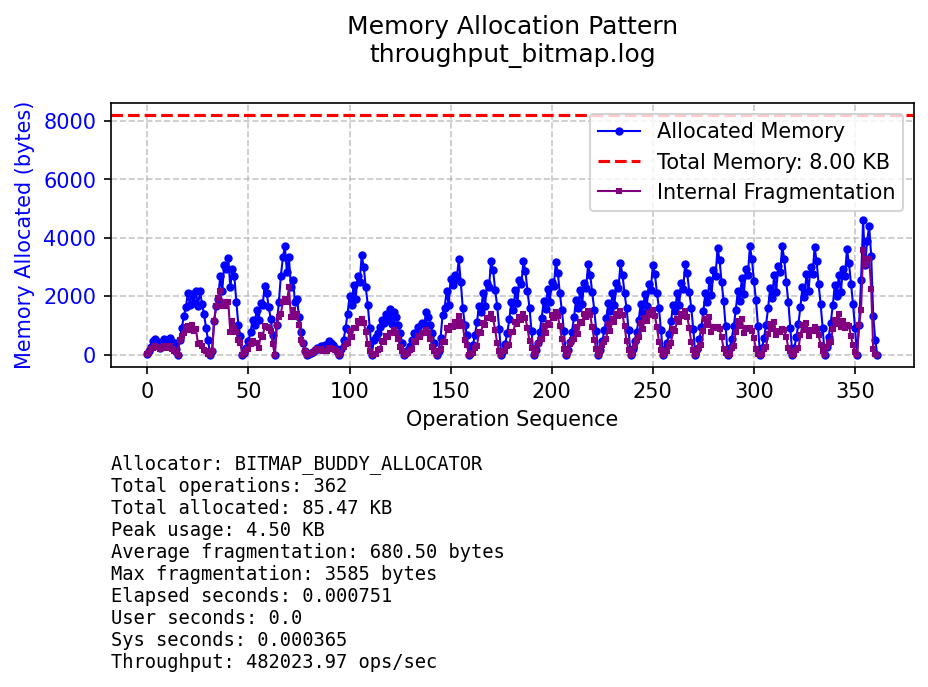
\includegraphics[width=0.9\textwidth]{graphs/throughput_bitmap.png}
  \label{fig:throughput_bitmap}
\end{figure}
\begin{lstlisting}[language={}]
I refs:        3,522,521
I1  misses:        2,786
LLi misses:        2,436
I1  miss rate:      0.08%
LLi miss rate:      0.07%

D refs:        1,744,339  (1,234,079 rd   + 510,260 wr)
D1  misses:        3,487  (    2,133 rd   +   1,354 wr)
LLd misses:        2,620  (    1,500 rd   +   1,120 wr)
D1  miss rate:       0.2% (      0.2%     +     0.3%  )
LLd miss rate:       0.2% (      0.1%     +     0.2%  )

LL refs:           6,273  (    4,919 rd   +   1,354 wr)
LL misses:         5,056  (    3,936 rd   +   1,120 wr)
LL miss rate:        0.1% (      0.1%     +     0.2%  )
\end{lstlisting}

\pagebreak

\subsection{Esempi di file \texttt{.alloc}}
\begin{lstlisting}[language={}]
% Tipo di allocatore (Slab)
i,slab         
% Parametri: slab_size=64, num_slabs=16
p,64,16        
% Alloca un blocco nell'indice 0
a,0            
% Alloca un blocco nell'indice 1
a,1            
% Libera il blocco nell'indice 0
f,0      
\end{lstlisting}      
\begin{lstlisting}[language={}]
% Benchmark per allocatore variabile
i,buddy
% memory_size=1024, max_levels=5
p,1024,5       
% Alloca 256 byte nell'indice 0
a,0,256        
% Alloca 128 byte nell'indice 1
a,1,128        
% Libera l'indice 0
f,0            
% Alloca 64 byte nell'indice 2
a,2,64         
\end{lstlisting}
\pagebreak




